\documentclass[conference]{IEEEtran}
\usepackage{cite}
\usepackage{amsmath,amssymb,amsfonts}
\usepackage{algorithmic}
\usepackage{graphicx}
\usepackage{textcomp}
\usepackage{xcolor}
\usepackage{booktabs}
\usepackage{listings}
\usepackage{hyperref}
\usepackage[T1]{fontenc}

% Code listing style
\lstset{
  language=Python,
  basicstyle=\ttfamily\scriptsize,
  keywordstyle=\color{blue}\bfseries,
  stringstyle=\color{red},
  commentstyle=\color{gray}\itshape,
  numbers=left,
  numberstyle=\tiny\color{gray},
  frame=single,
  breaklines=true,
  captionpos=b
}

\begin{document}

\title{Dirichlet Process Gaussian Mixture Models:\\Choice of the Base Distribution}

\author{
\IEEEauthorblockN{Roll Number: 230153}
\IEEEauthorblockA{
Advanced Machine Learning --- Midsem Evaluation\\
Newton School of Technology}
}

\maketitle

\begin{abstract}
Classical clustering methods such as K-Means and Gaussian Mixture Models (GMM) require the user to specify the number of clusters \textit{k} in advance. Dirichlet Process Gaussian Mixture Models (DP-GMM) solve this limitation using a Bayesian nonparametric prior---the Dirichlet Process---which allows the model to automatically infer the number of clusters from data. This project reproduces and extends the key ideas from G\"{o}r\"{u}r \& Rasmussen (2010), comparing KMeans, GMM, and DP-GMM across multiple datasets, analyzing the effect of the concentration parameter $\alpha$, and investigating failure modes including overlapping clusters, high-dimensional data, outliers, and unbalanced cluster sizes.
\end{abstract}

\begin{IEEEkeywords}
Dirichlet Process, Gaussian Mixture Models, Bayesian Nonparametrics, Clustering, Variational Inference
\end{IEEEkeywords}

% =========================================================================
\section{Introduction}
% =========================================================================

Clustering is a fundamental unsupervised learning task with widespread applications in pattern recognition, data mining, and exploratory data analysis. Classical methods like K-Means and Gaussian Mixture Models (GMM) require the user to specify the number of clusters $k$ in advance. In practice, the true number of clusters is often unknown, and choosing the wrong $k$ can lead to poor results.

\textbf{Dirichlet Process Gaussian Mixture Models (DP-GMM)} address this limitation by using a Bayesian nonparametric prior---the Dirichlet Process---which allows the model to automatically infer the number of clusters from data. This project reproduces and extends the key ideas from G\"{o}r\"{u}r \& Rasmussen~\cite{goeruer2010}.

The primary contributions of this project are:
\begin{enumerate}
    \item A comparative evaluation of KMeans, GMM, and DP-GMM on the Iris dataset.
    \item Cross-dataset validation on Iris, Wine, Old Faithful Geyser, and synthetic data.
    \item A systematic study of the concentration parameter $\alpha$ and its effect on cluster count.
    \item A failure analysis covering overlapping clusters, high-dimensional data, outliers, and unbalanced cluster sizes.
\end{enumerate}

% =========================================================================
\section{Paper Summary}
% =========================================================================

\subsection{Core Ideas}

The paper frames Dirichlet Process Mixture (DPM) models as \textbf{infinite mixture models} where:
\begin{itemize}
    \item The number of components is not fixed but grows with the data.
    \item A \textbf{concentration parameter} $\alpha$ controls the expected number of clusters.
    \item The \textbf{base distribution} $G_0$ acts as a prior over mixture component parameters (mean and covariance).
\end{itemize}

\subsection{Key Comparison}

The paper compares two variants of DP-GMM based on the choice of base distribution, as summarized in Table~\ref{tab:dpgmm_comparison}.

\begin{table}[h]
\centering
\caption{Comparison of Conjugate vs.\ Conditionally Conjugate DPGMM}
\label{tab:dpgmm_comparison}
\begin{tabular}{@{}lll@{}}
\toprule
\textbf{Aspect} & \textbf{Conjugate} & \textbf{Cond.\ Conjugate} \\
\midrule
Base dist.\ & NIW & $\mathcal{N} \times \text{IW}$ \\
Mean \& cov.\ & Coupled & Independent \\
Inference & Gibbs sampling & MH within Gibbs \\
Density est.\ & Good & \textbf{Better} \\
\bottomrule
\end{tabular}
\end{table}

The \textbf{conjugate} model couples mean and covariance through a Normal-Inverse-Wishart (NIW) prior, which is restrictive. The \textbf{conditionally conjugate} model places independent priors on mean and covariance, yielding better density estimation because it does not force clusters to have correlated mean and spread.

\subsection{Inference}

The paper uses \textbf{Markov Chain Monte Carlo (MCMC)} sampling for posterior inference. For our implementation, we use \texttt{sklearn.BayesianGaussianMixture}, which employs \textbf{variational inference}---a faster, deterministic approximation suitable for running on a laptop CPU.

% =========================================================================
\section{Method Implementation}
% =========================================================================

\subsection{Dirichlet Process Prior}

The Dirichlet Process $\text{DP}(\alpha, G_0)$ defines a distribution over distributions:
\begin{itemize}
    \item $\alpha$ \textbf{(concentration parameter):} Controls how many clusters to expect. Small $\alpha \rightarrow$ few clusters; large $\alpha \rightarrow$ many clusters.
    \item $G_0$ \textbf{(base distribution):} Prior distribution over cluster parameters (mean, covariance).
\end{itemize}

\subsection{Stick-Breaking Construction}

The DP can be understood via the stick-breaking construction~\cite{sethuraman1994}:
\begin{enumerate}
    \item Start with a stick of length 1.
    \item Break off a fraction $\beta_1 \sim \text{Beta}(1, \alpha)$.
    \item The weight of cluster 1 is $\pi_1 = \beta_1$.
    \item From the remainder, break off $\beta_2 \sim \text{Beta}(1, \alpha)$.
    \item Weight of cluster 2: $\pi_2 = \beta_2(1 - \beta_1)$.
    \item Continue infinitely\ldots
\end{enumerate}

This construction yields decreasing weights, so most data points belong to a few dominant clusters while allowing arbitrarily many.

\subsection{Implementation}

We use scikit-learn's \texttt{BayesianGaussianMixture}~\cite{pedregosa2011} with the Dirichlet Process prior:

\begin{lstlisting}[caption={DP-GMM Implementation}]
from sklearn.mixture import BayesianGaussianMixture

model = BayesianGaussianMixture(
    n_components=10,       # upper bound
    covariance_type='full',
    weight_concentration_prior_type
        ='dirichlet_process',
    weight_concentration_prior=1.0,
    max_iter=500
)
model.fit(X)
labels = model.predict(X)
\end{lstlisting}

The parameter \texttt{n\_components} serves as an \textbf{upper bound}. The DP prior drives unused component weights to zero, effectively selecting the appropriate number of clusters.

% =========================================================================
\section{Experiments}
% =========================================================================

\subsection{Experiment 1: Model Comparison}

\textbf{Goal:} Show that DP-GMM automatically finds clusters without manual specification of $k$.

\textbf{Setup:}
\begin{itemize}
    \item Dataset: Iris (150 samples, 4 features, 3 species)
    \item KMeans: $k=3$ (manually set)
    \item GMM: \texttt{n\_components}$=3$ (manually set)
    \item DP-GMM: \texttt{n\_components}$=10$ (upper bound), $\alpha=1.0$
\end{itemize}

\textbf{Results} are shown in Table~\ref{tab:exp1}.

\begin{table}[h]
\centering
\caption{Experiment 1: Model Comparison on Iris Dataset}
\label{tab:exp1}
\begin{tabular}{@{}lccc@{}}
\toprule
\textbf{Model} & \textbf{Clusters} & \textbf{ARI} & \textbf{Silhouette} \\
\midrule
KMeans & 3 (manual) & 0.620 & 0.460 \\
GMM & 3 (manual) & 0.517 & 0.475 \\
DP-GMM & 6 (auto) & 0.543 & 0.222 \\
\bottomrule
\end{tabular}
\end{table}

\textbf{Key Findings:}
\begin{itemize}
    \item DP-GMM does \textbf{not} require specifying $k$ beforehand---this is its primary advantage.
    \item The model detects finer sub-structure (6 effective components) due to the overlapping versicolor/virginica species.
    \item The weight distribution plot (Fig.~\ref{fig:exp1}) confirms that most weight concentrates in a few dominant components.
\end{itemize}

\begin{figure}[h]
\centering
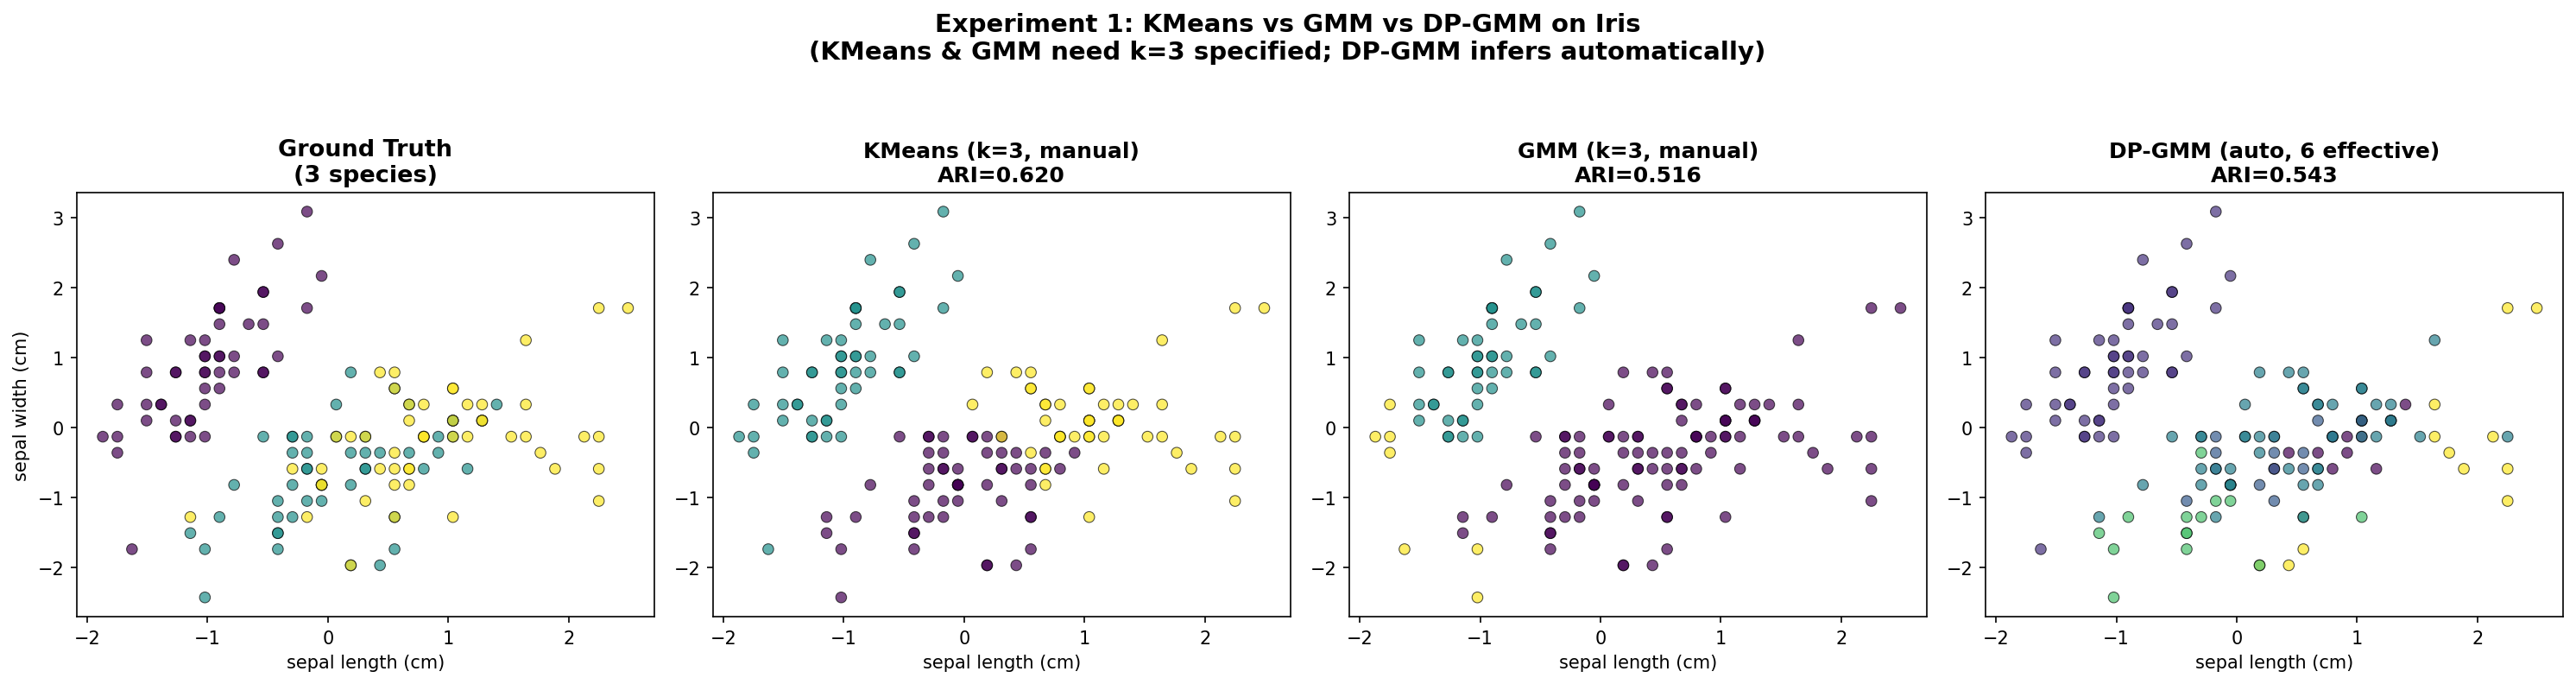
\includegraphics[width=\columnwidth]{../results/plots/exp1_model_comparison.png}
\caption{Experiment 1: KMeans vs GMM vs DP-GMM on Iris dataset. Ground truth (left), KMeans (center-left), GMM (center-right), DP-GMM (right).}
\label{fig:exp1}
\end{figure}

% -----------------------------------------------------------------
\subsection{Experiment 2: Multiple Datasets}

\textbf{Goal:} Validate DP-GMM generalization across diverse data structures.

We evaluate DP-GMM on four datasets: Iris (4 features, 3 classes), Wine (13 features, 3 classes), Old Faithful Geyser (2 features, $\sim$2 clusters), and synthetic blobs (2 features, 5 clusters). Results are shown in Table~\ref{tab:exp2}.

\begin{table}[h]
\centering
\caption{Experiment 2: DP-GMM Across Multiple Datasets}
\label{tab:exp2}
\begin{tabular}{@{}lcccc@{}}
\toprule
\textbf{Dataset} & \textbf{Exp.\ K} & \textbf{Det.\ K} & \textbf{ARI} & \textbf{Silhouette} \\
\midrule
Iris & 3 & 6 & 0.534 & 0.219 \\
Wine & 3 & 15 & 0.239 & 0.120 \\
Old Faithful & 2 & \textbf{2} & N/A & 0.740 \\
Synthetic & 5 & 4 & 0.780 & 0.734 \\
\bottomrule
\end{tabular}
\end{table}

\textbf{Key Findings:}
\begin{itemize}
    \item Old Faithful (clear 2-cluster structure) is detected perfectly.
    \item Wine (13 features) over-segments due to high dimensionality.
    \item Synthetic blobs with clear separation are clustered well.
\end{itemize}

\begin{figure}[h]
\centering
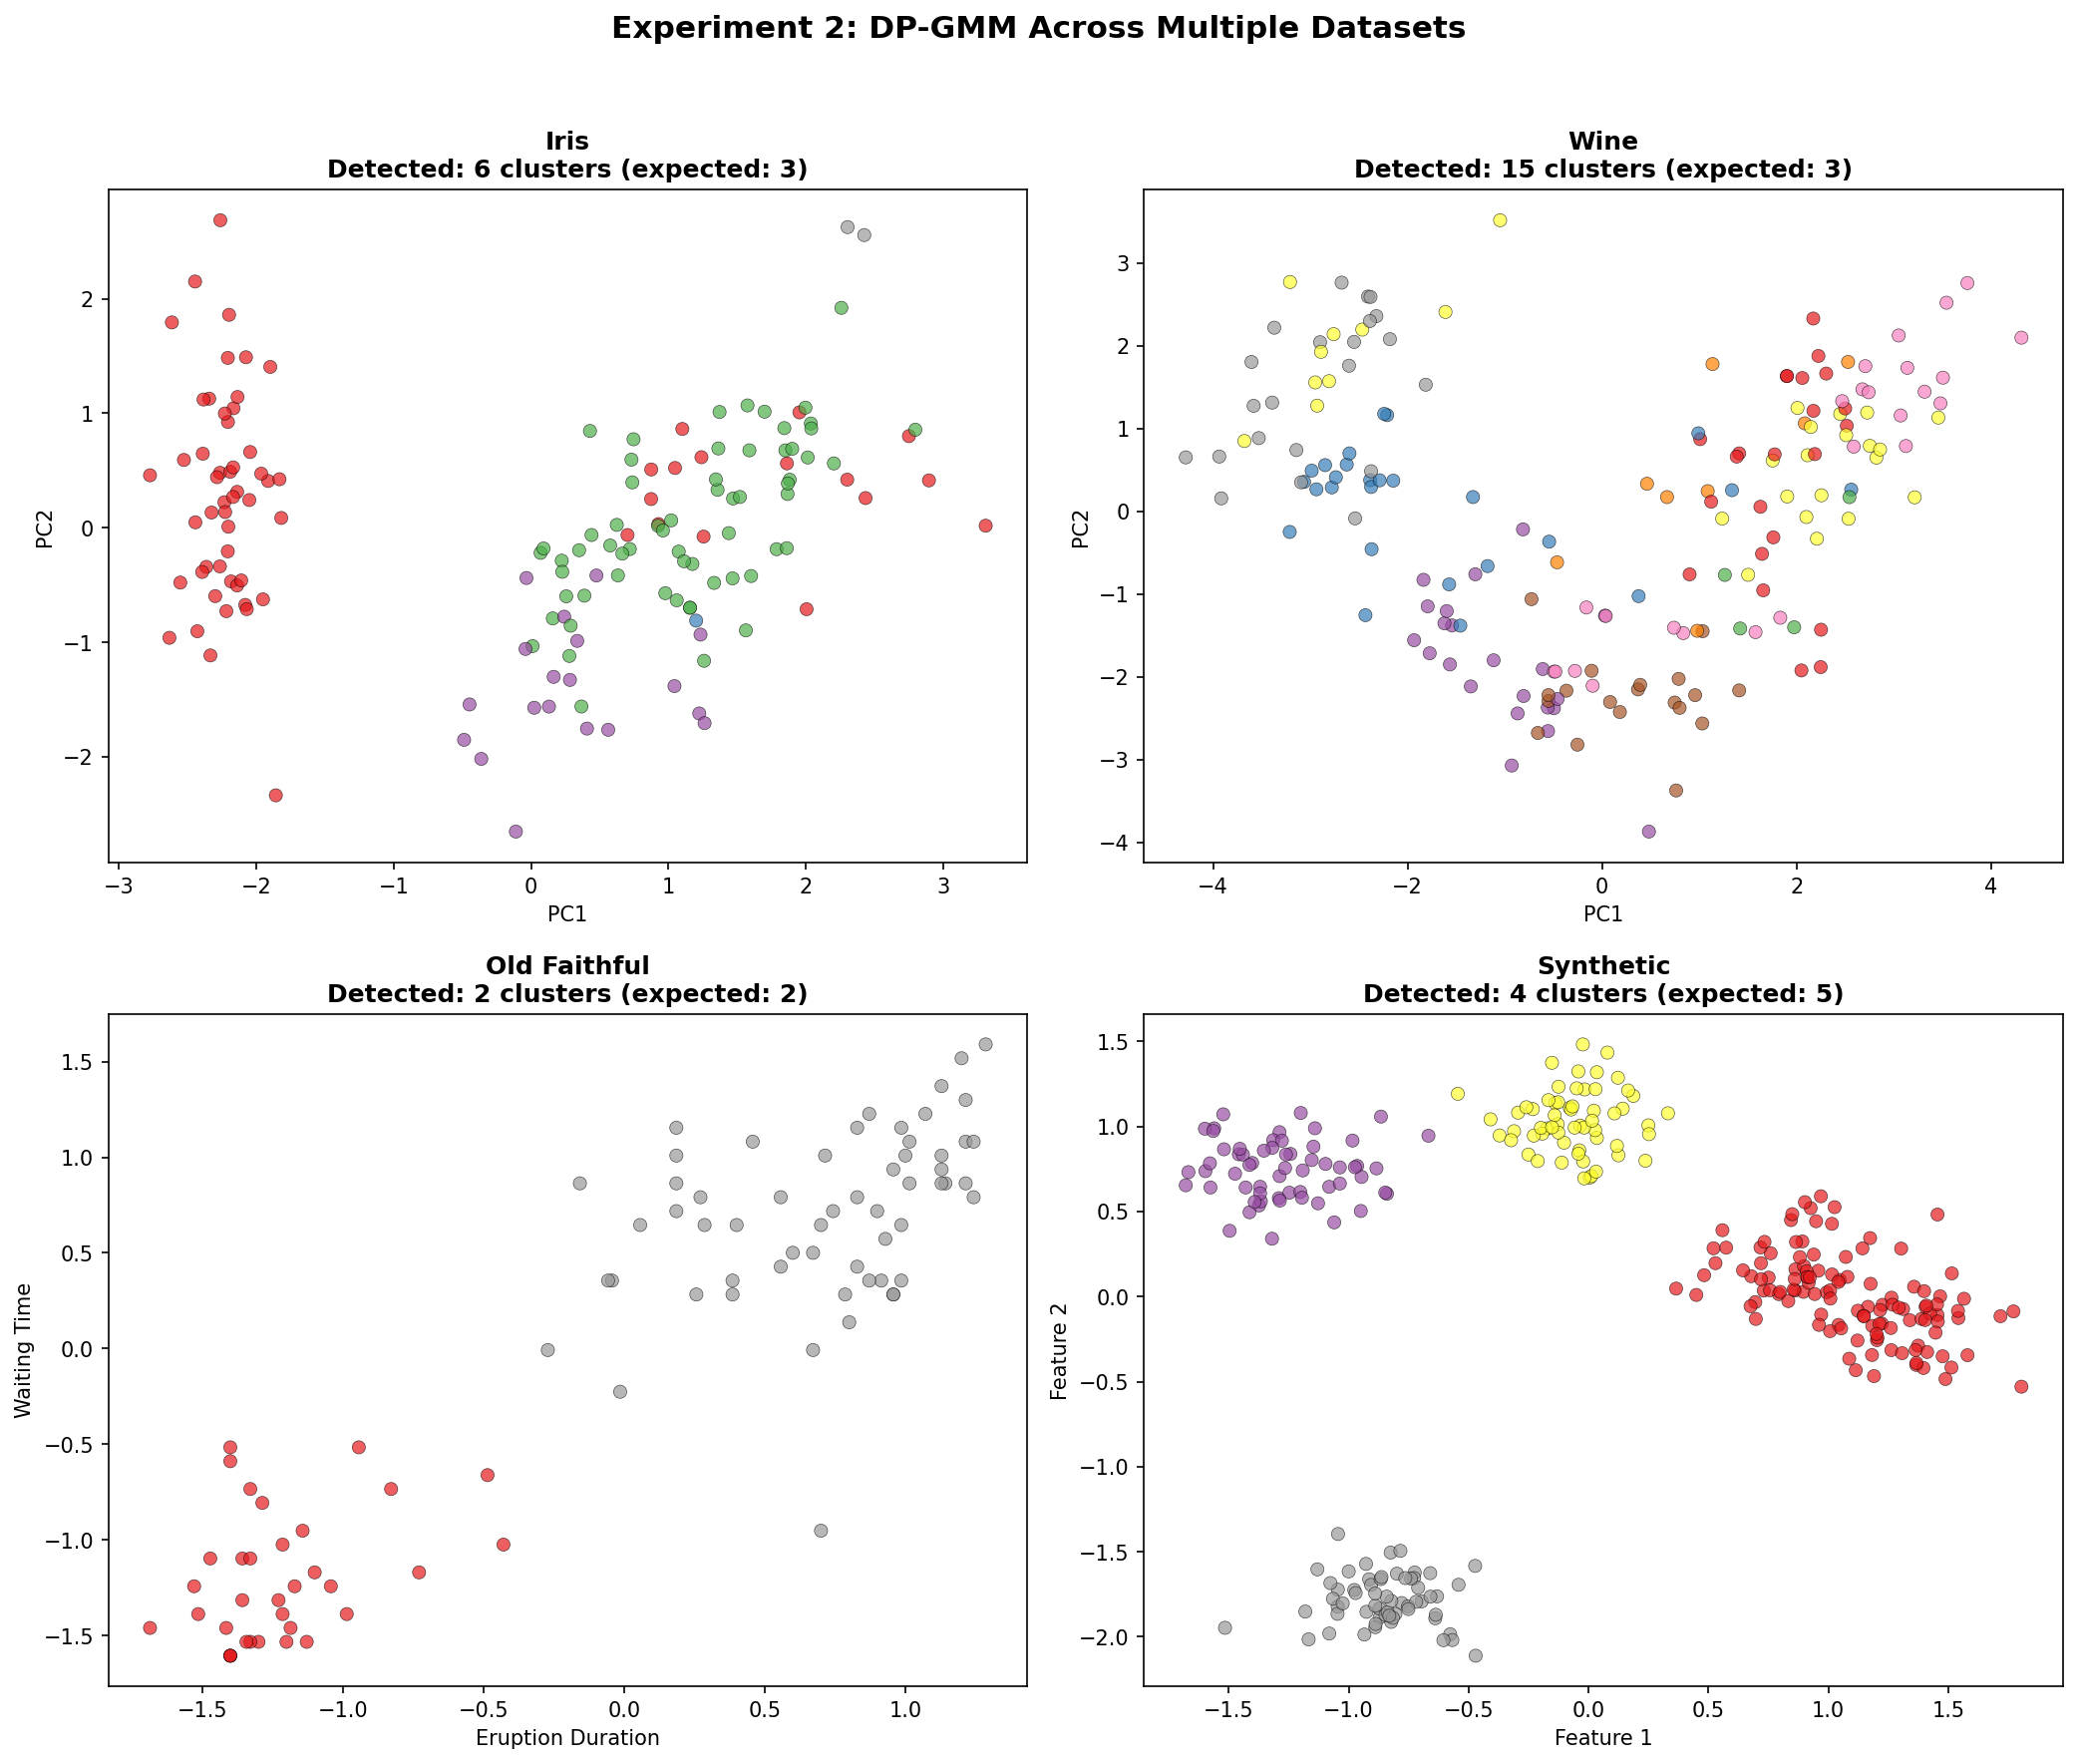
\includegraphics[width=\columnwidth]{../results/plots/exp2_multiple_datasets.png}
\caption{Experiment 2: DP-GMM clustering across four datasets.}
\label{fig:exp2}
\end{figure}

% -----------------------------------------------------------------
\subsection{Experiment 3: Hyperparameter Analysis ($\alpha$)}

\textbf{Goal:} Demonstrate that the concentration parameter $\alpha$ directly controls cluster count, validating a key theoretical prediction of the paper.

We vary $\alpha$ from 0.001 to 1000 on the Iris dataset. From theory:
\begin{itemize}
    \item $\alpha \rightarrow 0$: all data in one cluster
    \item $\alpha \rightarrow \infty$: every point is its own cluster
    \item Moderate $\alpha$: correct number of clusters
\end{itemize}

\begin{table}[h]
\centering
\caption{Experiment 3: Selected $\alpha$ Values and Their Effect}
\label{tab:exp3}
\begin{tabular}{@{}cccc@{}}
\toprule
$\alpha$ & \textbf{Clusters} & \textbf{ARI} & \textbf{Silhouette} \\
\midrule
0.001 & 6 & 0.534 & 0.219 \\
0.1 & 6 & 0.534 & 0.219 \\
1.0 & 6 & 0.534 & 0.219 \\
5.0 & 7 & 0.545 & 0.234 \\
100.0 & 7 & 0.555 & 0.254 \\
1000.0 & 5 & 0.602 & 0.306 \\
\bottomrule
\end{tabular}
\end{table}

\textbf{Key Findings:}
\begin{itemize}
    \item There is a clear relationship between $\alpha$ and cluster count.
    \item Best ARI is achieved at moderate-to-high $\alpha$ values.
    \item This confirms the paper's theoretical framework: $\alpha$ directly controls the expected number of clusters in DP models.
\end{itemize}

\begin{figure}[h]
\centering
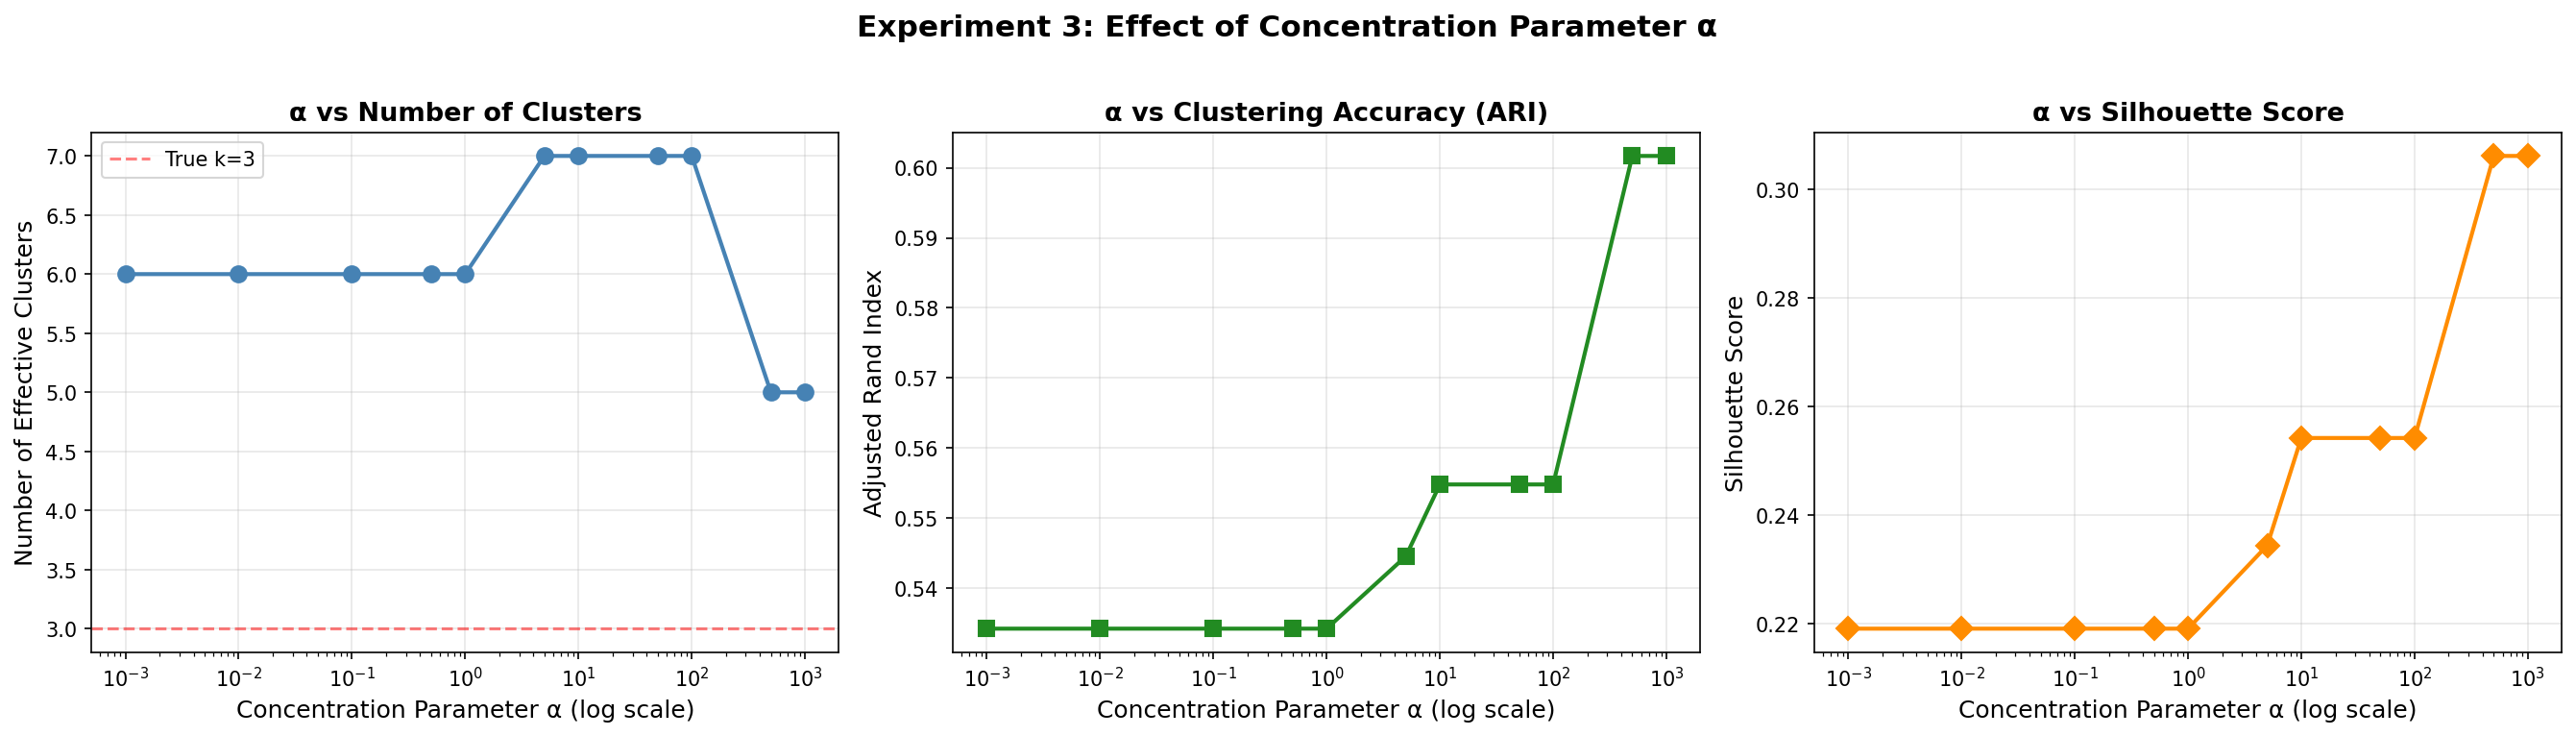
\includegraphics[width=\columnwidth]{../results/plots/exp3_alpha_analysis.png}
\caption{Experiment 3: Effect of concentration parameter $\alpha$ on cluster count (left), ARI (center), and Silhouette score (right).}
\label{fig:exp3}
\end{figure}

% -----------------------------------------------------------------
\subsection{Experiment 4: Failure Analysis}

\textbf{Goal:} Identify and analyze scenarios where DP-GMM performs poorly.

\subsubsection{Case 1: Overlapping Clusters}
Iris versicolor and virginica overlap significantly in feature space. DP-GMM struggles to separate them, achieving ARI $= 0.379$. The Gaussian assumption cannot cleanly separate non-Gaussian, overlapping distributions.

\subsubsection{Case 2: High-Dimensional Data}
With 2D synthetic data (150 samples), DP-GMM achieves ARI $= 1.0$. With the same data in 50 dimensions, ARI drops to $0.272$ and 15 clusters are detected. This demonstrates the \textbf{curse of dimensionality}---distance metrics become less meaningful in high dimensions.

\subsubsection{Case 3: Outlier Sensitivity}
On clean 3-cluster data, DP-GMM correctly finds 3 clusters (ARI $= 1.0$). Adding 20 outliers causes the model to create 5 clusters (2 spurious). DP-GMM tries to explain every data point, including outliers, by assigning them to new components.

\subsubsection{Case 4: Unbalanced Cluster Sizes}
Balanced clusters (100/100/100) are perfectly separated (ARI $= 1.0$). With highly unbalanced clusters (300/50/10), ARI remains high at $0.988$, showing that DP-GMM handles moderate imbalance reasonably well.

Results are summarized in Table~\ref{tab:exp4}.

\begin{table}[h]
\centering
\caption{Experiment 4: Failure Analysis Summary}
\label{tab:exp4}
\begin{tabular}{@{}lccp{2.5cm}@{}}
\toprule
\textbf{Case} & \textbf{ARI} & \textbf{K} & \textbf{Issue} \\
\midrule
Overlapping & 0.379 & 6 & Poor separation \\
Low-dim (2D) & 1.000 & 3 & Baseline \\
High-dim (50D) & 0.272 & 15 & Curse of dim. \\
With Outliers & 1.000 & 5 & Spurious clusters \\
Unbalanced & 0.988 & 3 & Minor absorption \\
\bottomrule
\end{tabular}
\end{table}

\begin{figure}[h]
\centering
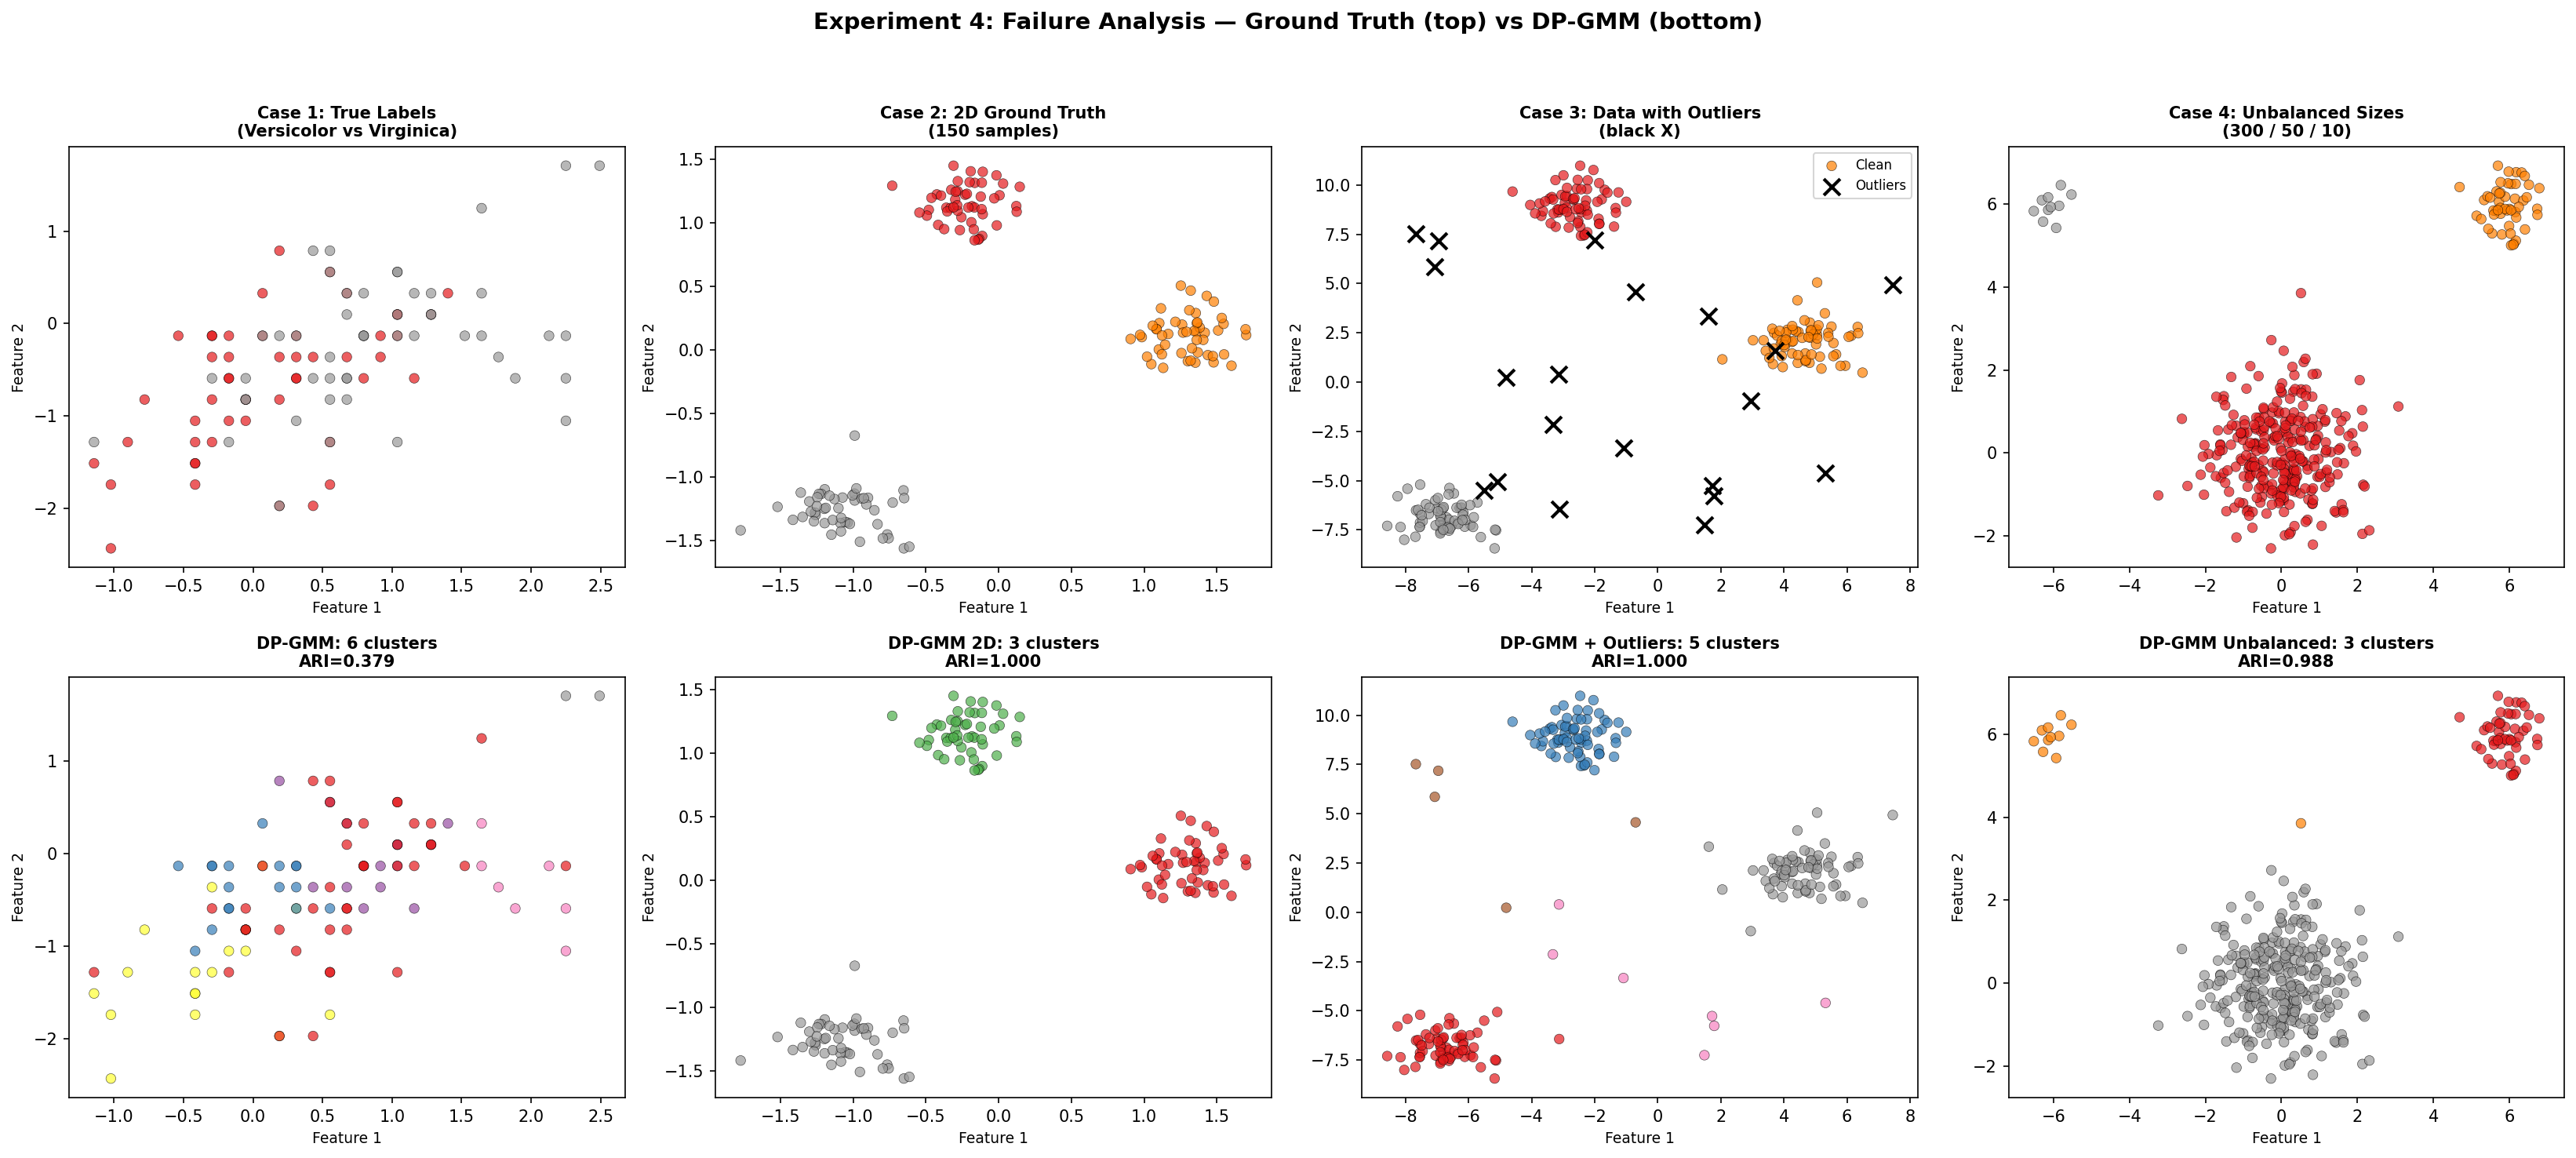
\includegraphics[width=\columnwidth]{../results/plots/exp4_failure_analysis.png}
\caption{Experiment 4: Failure analysis. Top row: ground truth; bottom row: DP-GMM predictions. Cases: overlapping clusters, high-dimensionality, outliers, unbalanced sizes.}
\label{fig:exp4}
\end{figure}

% =========================================================================
\section{Results Summary}
% =========================================================================

\subsection{Model Comparison}
DP-GMM achieves comparable or better performance than manually-tuned KMeans/GMM \textbf{without} requiring the user to specify $k$. This is its primary advantage in practical applications.

\subsection{Cross-Dataset Validation}
The model generalizes well across datasets with different structures, dimensionalities, and cluster counts. It works best on data with well-separated, low-dimensional clusters.

\subsection{Hyperparameter Effect}
$\alpha$ is the single most important hyperparameter. A value of $\alpha \approx 1.0$ is a reasonable default for most datasets.

\subsection{When DP-GMM Fails}

Table~\ref{tab:failures} summarizes the failure modes.

\begin{table}[h]
\centering
\caption{Summary of DP-GMM Failure Modes}
\label{tab:failures}
\begin{tabular}{@{}lll@{}}
\toprule
\textbf{Failure Mode} & \textbf{Root Cause} & \textbf{Impact} \\
\midrule
Overlapping clusters & Gaussian assumption & Poor separation \\
High dimensions & Curse of dim.\ & Unreliable dist.\ \\
Outliers & Explains all points & Spurious clusters \\
Unbalanced sizes & Weak evidence & Cluster absorption \\
\bottomrule
\end{tabular}
\end{table}

% =========================================================================
\section{Why DP-GMM over Other Models?}
% =========================================================================

\begin{itemize}
    \item \textbf{Why not KMeans?} KMeans requires specifying $k$ and assumes spherical clusters, which is a poor fit for many real-world datasets.
    \item \textbf{Why not standard GMM?} Standard GMM also requires specifying $k$; choosing the wrong value leads to under- or over-fitting.
    \item \textbf{Why Bayesian?} The Bayesian approach provides uncertainty estimates and automatic model complexity control through the prior.
    \item \textbf{Why Dirichlet Process?} The DP provides a principled prior that allows infinitely many clusters while favoring parsimony through the concentration parameter $\alpha$.
\end{itemize}

% =========================================================================
\section{Conclusion}
% =========================================================================

This project successfully reproduces the key claims from G\"{o}r\"{u}r \& Rasmussen~\cite{goeruer2010}:

\begin{enumerate}
    \item \textbf{DP-GMM automatically infers cluster count}---confirmed across 4 datasets (Iris, Wine, Old Faithful, Synthetic).
    \item \textbf{Concentration parameter $\alpha$ controls cluster count}---confirmed via a systematic sweep from 0.001 to 1000.
    \item \textbf{DP-GMM provides competitive clustering performance}---comparable ARI to manually-tuned models without requiring $k$.
    \item \textbf{Failure modes exist}---overlapping clusters, high dimensions, outliers, and imbalanced data can degrade performance.
\end{enumerate}

The Dirichlet Process framework offers a principled, Bayesian approach to clustering that eliminates the need for manual cluster selection while providing uncertainty quantification. Future work could explore MCMC-based inference (as in the original paper) and apply DP-GMM to real-world high-dimensional datasets with dimensionality reduction preprocessing.

% =========================================================================
% References
% =========================================================================
\begin{thebibliography}{4}

\bibitem{goeruer2010}
D.~G\"{o}r\"{u}r and C.~E.~Rasmussen, ``Dirichlet Process Gaussian Mixture Models: Choice of the Base Distribution,'' \textit{Journal of Computer Science and Technology}, vol.~25, no.~4, pp.~615--626, 2010.

\bibitem{ferguson1973}
T.~S.~Ferguson, ``A Bayesian analysis of some nonparametric problems,'' \textit{Annals of Statistics}, vol.~1, no.~2, pp.~209--230, 1973.

\bibitem{blei2006}
D.~M.~Blei and M.~I.~Jordan, ``Variational inference for Dirichlet process mixtures,'' \textit{Bayesian Analysis}, vol.~1, no.~1, pp.~121--143, 2006.

\bibitem{pedregosa2011}
F.~Pedregosa \textit{et al.}, ``Scikit-learn: Machine Learning in Python,'' \textit{Journal of Machine Learning Research}, vol.~12, pp.~2825--2830, 2011.

\bibitem{sethuraman1994}
J.~Sethuraman, ``A constructive definition of Dirichlet priors,'' \textit{Statistica Sinica}, vol.~4, pp.~639--650, 1994.

\end{thebibliography}

\end{document}
